\chapter{Gamma-ray Astronomy }
\label{chap:gamAstr}

\begin{figure}[h!]%[t] 
	\centering
	\makebox[\linewidth]{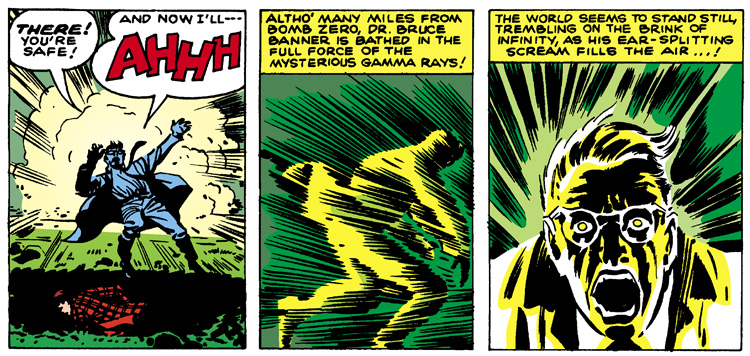
\includegraphics[width=1.\columnwidth]{Figures/panel_hulk001b}}
\end{figure}

%\begin{quote}
%	``Once there was a boy, and the boy loved stars very much'' 
%	\begin{center}---by Oliver Jeffers, from \it{How to Catch a Star} \end{center}
%\end{quote}


%ugh commentes
%\section{Introduction}\label{gamAstr:intro}


\section{\gam{} Emission Mechanisms }\label{gamAstr:Emiss}
The story of \gam{}s from astrophysical objects is a tale of the most extreme, energetic, and violent environments in our universe. \gam{}s are the highest named energy of light ranging from energies of order and\mev{} extending up with the highest detected energies up to  hundreds of \tev{}. Aside from the  nuclear decay of heavy particles, \gam{}s are produced solely by charged particles being accelerated to\gev{} and\tev{} energies and interacting either with a target particle, be it other matter or photon fields.  Below we summarize the various non-thermal emission mechanisms giving rise to \gam{}s, namely, \ic{} radiation, non-thermal \brems{} (both of an accelerated electron, or leptionic, origin), and neutral pion decay emission (of an accelerated proton, or hadronic origin). We also described the \sync{} radiation process. While not typically observed up to \gam{} energies (with \sync{}  emission from the Crab nebula being an exception \cite{AbdoCrab}, with the tail of the emission extending to hundreds of\mev{}), \sync{} photons plays a significant role in understanding \ic{} \gam{} emission since the processes both arise from a shared, underlying electron population. Furthermore, observations of \sync{} emission at radio and X-ray energies is vital in  constraining a source's underlying charged particle population and the resultant \gam{} source spectra. We follow \cite{Houck06} for many of the photon emissivities given below.

\subsection{Synchrotron Radiation}\label{gamAstr:sync}
When a relativistic electron moves in a magnetic field, it experiences a force perpendicular to its velocity which causes the electron to accelerate and travel in a helical path around the magnetic field lines. This acceleration results in radiation of photons, referred to as \sync{} radiation \cite{Blumenthal70,Pacholczyk70,Rybicki86,Longair11}. The total power emitted at frequency $\nu$ from a relativistic electron (Lorentz factor, $\gamma \gg 1$) spiraling in a magnetic field, B, is given as:

\begin{equation}\label{eq:syncPow}
{\rm P_{emitted}(\nu) = 
\frac{\sqrt{3} q^3 B \sin\alpha}{m_e c^2} F(\nu/\nu_c) }
\end{equation}
where q is the electron's charge,  ${\rm m_e}$ the electron's rest mass, c the speed of light,  ${\rm \alpha }$ the angle between the magnetic field vector and the electron's velocity vector (the pitch angle), and the critical frequency, the frequency at which most of the power is radiated is given as:

\begin{equation}\label{eq:nuCrit}
\nu_c = \frac{3q B \gamma^2}{4\pi m_e c} 
\sin\alpha \equiv \nu_0 \gamma^2 \sin\alpha
\end{equation}
and F, called the first synchrotron function, is an integral over an irregular modified Bessel function (see \cite{Rybicki86}). We note that the power emitted is inversely proportional to the mass, which explains the insignificance of proton synchrotron radiation, where the rest mass of the proton is $\sim$ 2000 times greater than that of the electron.

For an isotropic distribution of electrons we define  ${\rm N(p,\alpha)}$ as the number of electrons per unit solid angle and momentum with momentum p and pitch angle $\alpha$. \cite{Houck06} show that the differential photon-emissivity spectrum (\ie{}\ number of radiated photons per unit time per unit energy) is:

\begin{equation}
\frac{d n}{d \omega d t} =
\frac{\sqrt{3}q^3 B}{h m_e c^2 \nu}
\int
N(p)
R \left(\frac{\omega}{\omega_0 \gamma^2}\right)dp
\end{equation}
with $\omega$ being the radiated photon energy, ${\rm N(p) = 4\pi N(p,\alpha)}$ for an isotropic pitch-angle distribution, and
\begin{equation}
R(x) \equiv \frac{1}{2} \int_0^\pi
\sin^2 \alpha
F\left(\frac{x}{\sin\alpha}\right) d \alpha 
\end{equation}


\subsection{Non-Thermal \brems{}}\label{gamAstr:bremss}
Bremsstrahlung radiation occurs when charged particles (electron-electron or electron-ion in this case) pass near each other, causing the  primary charge to decelerate, and emit a photon. For a differential spectrum, ${\rm N_e(p)}$, corresponding to the accelerated electrons, the total emissivity is given as the sum of the electron-electron and electron-ion \brems{}. The combined differential photon-emissivity spectrum can be given as:

\begin{equation}
{\rm \frac{d n}{d \omega d t} =
	n_e \int
	N_e(p) v_e
	\frac{d \sigma_{e e}}{d \omega}dp +
	n_Z \int
	N_e(p) v_e
	\frac{d \sigma_{e Z}}{d \omega}dp}
\end{equation}
where ${\rm d \sigma_{e Z}/d \omega}$ and ${\rm d \sigma_{e e}/d \omega}$ are the differential interaction cross sections for each interaction \citep{Koch59,Haug75}, ${\rm n_e}$ and ${\rm n_Z}$ are the stationary electron and ion densities, and ${\rm v_e}$ is the electron velocity.

\subsection{Inverse Compton Scattering}\label{gamAstr:IC}

\ic{} scattering refers to the process by which a high-energy electron collides with a lower-energy photon transferring energy and ``upscattering" the photon to higher energies \citep{Blumenthal70}. The dominant seed photon field available for upscattering by a population of electrons is that of the \cmb{}, with a temperature ${\rm T \approx 2.73~K}$. Other photon fields that may be relevant are \fir{} dust emission (${\rm T \approx 30~K}$), and \nir{} stellar-light (${\rm T \approx 3000~K}$). For a thermal photon-field of number density $n(\omega_i)$, with $\omega_i$ being the incident and photon energy,

\begin{equation}
n(\omega_i) = 
\frac{1}{\pi^2\lambda^3} 
\frac{\omega_i^2}{e^{\omega_i/\Theta} -1}
\end{equation}
where  $\Theta=kT/(m_e c^2)$, and the Compton wavelength of the electron is $\lambda=\hbar/(m_e c)$.
For a momentum distribution of relativistic electrons, ${\rm N_e(p)}$, embedded in an isotropic photon-field of number density $n(\omega_i)$, the single-photon differential photon-emissivity spectrum,  is given by:

\begin{equation}
{\rm \frac{dn}{d\omega dt} = 
c \int  n(\omega_i)d \omega_i
\int_{p_{min}}^\infty 
N_e(p)  \sigma_{KN}(\gamma,\omega_i,\omega)dp}
\end{equation}
with $\omega$ as the upscattered photon energy, ($\omega\equiv h\nu/(m_e c^2)$), and $\sigma_{KN}$ is the Klein-Nishina scattering  cross section:
\begin{equation}
{\rm \sigma_{KN}(\gamma,\omega_i,\omega) = \frac{2\pi r_0^2}{\omega_i \gamma^2}
\left[
1 + q - 2q^2 + 2q\ln q + \frac{\Gamma^2 q^2 (1-q)}{2(1+\Gamma q)}
\right]}
\end{equation}
and,
\begin{equation}
{\rm q \equiv \frac{\omega}{4 \omega_i \gamma (\gamma-\omega)}}
\end{equation}
for ${\rm \Gamma \equiv 4\omega_i \gamma}$, and the classical elec(as in \cite{Houck06})tron radius, ${\rm r_0 = e^2/(m_e c^2)}$

%\jamie{We note that in the Thomson limit, ${\rm \omega_i \ll omega \ll \gamma mc^2}$ the Klein-Nishina cross section reduces to the Thomson cross section. }


\subsection{Neutral Pion Decay Emission}\label{gamAstr:PP}
When high-energy protons and ions collide with interstellar material, one of the products of the collision is a neutral pion. The neutral pion subsequently (and expediently; within $~10^{-16}$ s) decays into two \gam{} photons, each of rest energy $\omega_0 =(m_{\pi}c^2)/2\approx 67.5\mev{}$. For a differential proton distribution ${\rm N_p(p)}$, the differential photon distribution is given by:

\begin{equation}
\frac{d n}{d \omega d t} = 
n_p \int v_p N_p(p) 
\frac{d \sigma(p_\pi, p)}{d p}dp
\end{equation}
where ${\rm n_p}$ is the density of the target protons, ${\rm d \sigma(p_\pi, p)/dp}$ the differential cross section for neutral pion production for proton collisions, and ${\rm v_p}$ the non-thermal proton velocity \citep{Hillier84,Dermer86,Aharonian00}. The peak of the distribution occurs at $\approx 68\mev{}$ , however the peak is broadened due to Doppler shifting of the momentum distribution of the high-energy protons. This feature shows a bilateral symmetry about the peak energy in a photon spectrum representation, but in a ${\rm \nu F_\nu}$ representation, it appears as a hardening of the spectrum at a few hundred\mev{} \cite{Stecker71,Dermer13}. This characteristic pion-decay feature is colloquially referred to as the ``pion-bump", and is a vital instrument in distinguishing the proton-emitting population from the often-overlapping \ic{} and \brems{} spectrum produced at \gam{}s. 

%\section{Sources of \gam's}\label{gamAstr:Sources}
\jamie{]write about gamma ray sky, diffuse, talk about other catalogs! variety of sources pie chart sources we see
\twofgl{} \threefgl{} \onefhl{} \twopc{} tev pwn cat}


%\section{\gam{} Observations}\label{gamAstr:obs}

\jamie{when I get to \egret{}}
